%\nonstopmode
\documentclass[aspectratio=169]{beamer}
\usepackage[utf8]{inputenc}
% \usepackage[frenchb]{babel}
\usepackage{amsmath}
\usepackage{mathtools}
\usepackage{breqn}
\usepackage{multirow}
\usetheme{boxes}
\usepackage{graphicx}
\usepackage{adjustbox}
%\useoutertheme[footline=authortitle,subsection=false]{miniframes}
%\useoutertheme[footline=authorinstitute,subsection=false]{miniframes}
\useoutertheme{infolines}
\setbeamertemplate{headline}{}

\beamertemplatenavigationsymbolsempty

\definecolor{TitleOrange}{RGB}{255,137,0}
\setbeamercolor{title}{fg=TitleOrange}
\setbeamercolor{frametitle}{fg=TitleOrange}

\definecolor{ListOrange}{RGB}{255,145,5}
\setbeamertemplate{itemize item}{\color{ListOrange}$\blacktriangleright$}

\definecolor{verygrey}{RGB}{70,70,70}
\setbeamercolor{normal text}{fg=verygrey}


\usepackage{tabu}
\usepackage{multicol}
\usepackage{vwcol}
\usepackage{stmaryrd}
\usepackage{graphicx}

\usepackage[normalem]{ulem}

\title{Introducing Garage}
\subtitle{a new storage platform for self-hosted geo-distributed clusters}
\author{Deuxfleurs Association}
\date{IMT Atlantique, 2022-06-23}

\begin{document}

\begin{frame}
	\centering
	\includegraphics[width=.3\linewidth]{../../sticker/Garage.pdf}
	\vspace{1em}

	{\large\bf Deuxfleurs Association}
	\vspace{1em}

	\url{https://garagehq.deuxfleurs.fr/}

	Matrix channel: \texttt{\#garage:deuxfleurs.fr}
\end{frame}

\begin{frame}
	\frametitle{Who we are}
	\begin{columns}[t]
		\begin{column}{.2\textwidth}
			\centering
			\adjincludegraphics[width=.4\linewidth, valign=t]{assets/alex.jpg}
		\end{column}
		\begin{column}{.6\textwidth}
			\textbf{Alex Auvolat}\\
			PhD at Inria, team WIDE; co-founder of Deuxfleurs
		\end{column}
		\begin{column}{.2\textwidth}
			~
		\end{column}
	\end{columns}
	\vspace{1em}

	\begin{columns}[t]
		\begin{column}{.2\textwidth}
			~
		\end{column}
		\begin{column}{.6\textwidth}
			\textbf{Quentin Dufour}\\
			PhD at Inria, team WIDE; co-founder of Deuxfleurs
		\end{column}
		\begin{column}{.2\textwidth}
			\centering
			\adjincludegraphics[width=.5\linewidth, valign=t]{assets/quentin.jpg}
		\end{column}
	\end{columns}
	\vspace{2em}

	\begin{columns}[t]
		\begin{column}{.2\textwidth}
			\centering
			\adjincludegraphics[width=.5\linewidth, valign=t]{assets/deuxfleurs.pdf}
		\end{column}
		\begin{column}{.6\textwidth}
			\textbf{Deuxfleurs}\\
			A non-profit self-hosting collective,\\
			member of the CHATONS network
		\end{column}
		\begin{column}{.2\textwidth}
			\centering
			\adjincludegraphics[width=.7\linewidth, valign=t]{assets/logo_chatons.png}
		\end{column}
	\end{columns}

\end{frame}

\begin{frame}
	\frametitle{Our objective at Deuxfleurs}
	
	\begin{center}
		\textbf{Promote self-hosting and small-scale hosting\\
			as an alternative to large cloud providers}
	\end{center}
	\vspace{2em}
	\visible<2->{
		Why is it hard?
	}
	\visible<3->{
		\vspace{2em}
		\begin{center}
			\textbf{\underline{Resilience}}\\
			{\footnotesize (we want good uptime/availability with low supervision)}
		\end{center}
	}
\end{frame}

\begin{frame}
	\frametitle{How to make a \underline{stable} system}

	Enterprise-grade systems typically employ:
	\vspace{1em}
	\begin{itemize}
		\item RAID
		\item Redundant power grid + UPS
		\item Redundant Internet connections
		\item Low-latency links
		\item ... 
	\end{itemize}
	\vspace{1em}
	$\to$ it's costly and only worth it at DC scale
\end{frame}

\begin{frame}
	\frametitle{How to make a \underline{resilient} system}

	\only<1,4-5>{
		Instead, we use:
		\vspace{1em}
		\begin{itemize}
			\item \textcolor<2->{gray}{Commodity hardware (e.g. old desktop PCs)}
				\vspace{.5em}
			\item<4-> \textcolor<5->{gray}{Commodity Internet (e.g. FTTB, FTTH) and power grid}
				\vspace{.5em}
			\item<5-> \textcolor<6->{gray}{\textbf{Geographical redundancy} (multi-site replication)}
		\end{itemize}
	}
	\only<2>{
		\begin{center}
			\includegraphics[width=.8\linewidth]{assets/atuin.jpg}
		\end{center}
	}
	\only<3>{
		\begin{center}
			\includegraphics[width=.8\linewidth]{assets/neptune.jpg}
		\end{center}
	}
	\only<6>{
		\begin{center}
			\includegraphics[width=.5\linewidth]{assets/inframap.jpg}
		\end{center}
	}
\end{frame}

\begin{frame}
	\frametitle{How to make this happen}
	\begin{center}
		\only<1>{\includegraphics[width=.8\linewidth]{assets/slide1.png}}%
		\only<2>{\includegraphics[width=.8\linewidth]{assets/slide2.png}}%
		\only<3>{\includegraphics[width=.8\linewidth]{assets/slide3.png}}%
	\end{center}
\end{frame}

\begin{frame}
	\frametitle{Distributed file systems are slow}
	File systems are complex, for example:
	\vspace{1em}
	\begin{itemize}
		\item Concurrent modification by several processes
			\vspace{1em}
		\item Folder hierarchies
			\vspace{1em}
		\item Other requirements of the POSIX spec
	\end{itemize}
	\vspace{1em}
	Coordination in a distributed system is costly

	\vspace{1em}
	Costs explode with commodity hardware / Internet connections\\
	{\small (we experienced this!)}
\end{frame}

\begin{frame}
	\frametitle{A simpler solution: object storage}
	Only two operations:
	\vspace{1em}
	\begin{itemize}
		\item Put an object at a key
			\vspace{1em}
		\item Retrieve an object from its key
	\end{itemize}
	\vspace{1em}
	{\footnotesize (and a few others)}

	\vspace{1em}
	Sufficient for many applications!
\end{frame}

\begin{frame}
	\frametitle{A simpler solution: object storage}
		\begin{center}
			\includegraphics[width=.2\linewidth]{../2020-12-02_wide-team/img/Amazon-S3.jpg}
			\hspace{5em}
			\includegraphics[width=.2\linewidth]{assets/minio.png}
		\end{center}
		\vspace{1em}
	S3: a de-facto standard, many compatible applications

	\vspace{1em}

	MinIO is self-hostable but not suited for geo-distributed deployments
\end{frame}


\begin{frame}
	\frametitle{But what is Garage, exactly?}
	\textbf{Garage is a self-hosted drop-in replacement for the Amazon S3 object store}\\
	\vspace{.5em}
	that implements resilience through geographical redundancy on commodity hardware
		\begin{center}
			\includegraphics[width=.8\linewidth]{assets/garageuses.png}
		\end{center}
\end{frame}

\begin{frame}
	\frametitle{Overview}
	\begin{center}
		\only<1>{\includegraphics[width=.45\linewidth]{assets/garage2a.drawio.pdf}}%
		\only<2>{\includegraphics[width=.45\linewidth]{assets/garage2b.drawio.pdf}}%
	\end{center}
\end{frame}

\begin{frame}
	\frametitle{Garage is \emph{location-aware}}
	\begin{center}
		\includegraphics[width=\linewidth]{assets/location-aware.png}
	\end{center}
	\vspace{2em}
	Garage replicates data on different zones when possible
\end{frame}

\begin{frame}
	\frametitle{Garage is \emph{location-aware}}
		\begin{center}
			\includegraphics[width=.8\linewidth]{assets/map.png}
		\end{center}
\end{frame}

\begin{frame}
	\frametitle{How to spread files over different cluster nodes?}
	\textbf{Consistent hashing (DynamoDB):}
	\vspace{1em}

	\begin{center}
	\only<1>{\includegraphics[width=.45\columnwidth]{assets/consistent_hashing_1.pdf}}%
	\only<2>{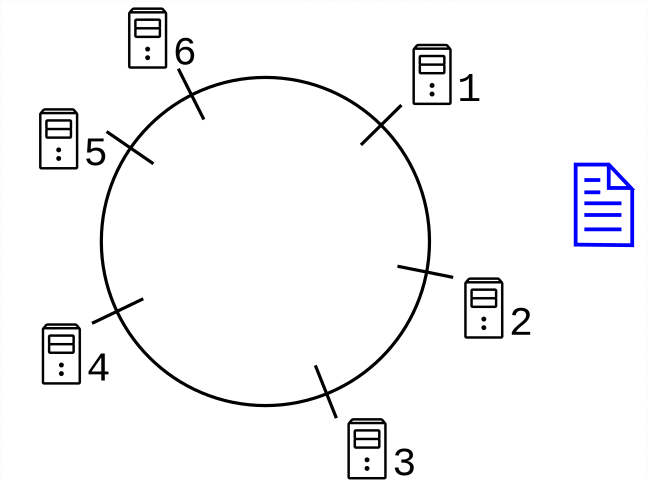
\includegraphics[width=.45\columnwidth]{assets/consistent_hashing_2.pdf}}%
	\only<3>{\includegraphics[width=.45\columnwidth]{assets/consistent_hashing_3.pdf}}%
	\only<4>{\includegraphics[width=.45\columnwidth]{assets/consistent_hashing_4.pdf}}%
	\end{center}
\end{frame}

\begin{frame}
	\frametitle{How to spread files over different cluster nodes?}
	\textbf{Issues with consistent hashing:}
	\vspace{1em}
	\begin{itemize}
		\item Doesn't dispatch data based on geographical location of nodes
			\vspace{1em}
		\item<2-> Geographically aware adaptation, try 1:\\
			data quantities not well balanced between nodes
			\vspace{1em}
		\item<3-> Geographically aware adaptation, try 2:\\
			too many reshuffles when adding/removing nodes
	\end{itemize}
\end{frame}

\begin{frame}
	\frametitle{How to spread files over different cluster nodes?}
	\textbf{Garage's method: build an index table}
	\vspace{1em}

	Realization: we can actually precompute an optimal solution
	\vspace{1em}

	\visible<2->{
		\begin{center}
		\begin{tabular}{|l|l|l|l|}
			\hline
			\textbf{Partition} & \textbf{Node 1} & \textbf{Node 2} & \textbf{Node 3} \\
			\hline
			\hline
			Partition 0 & Io (jupiter) & Drosera (atuin) & Courgette (neptune) \\
			\hline
			Partition 1 & Datura (atuin) & Courgette (neptune) & Io (jupiter) \\
			\hline
			Partition 2 & Io(jupiter) & Celeri (neptune) & Drosera (atuin) \\
			\hline
			\hspace{1em}$\vdots$ & \hspace{1em}$\vdots$ & \hspace{1em}$\vdots$ & \hspace{1em}$\vdots$ \\
			\hline
			Partition 255 & Concombre (neptune) & Io (jupiter) & Drosera (atuin) \\
			\hline
		\end{tabular}
		\end{center}
	}
	\vspace{1em}
	\visible<3->{
		The index table is built centrally using an optimal* algorithm,\\
		then propagated to all nodes\\
		\hfill\footnotesize *not yet optimal but will be soon
	}
\end{frame}

\begin{frame}
	\frametitle{Garage's internal data structures}
	\centering
	\includegraphics[width=.75\columnwidth]{assets/garage_tables.pdf}
\end{frame}

%\begin{frame}
%	\frametitle{Garage's architecture}
%	\begin{center}
%		\includegraphics[width=.35\linewidth]{assets/garage.drawio.pdf}
%	\end{center}
%\end{frame}

\begin{frame}
	\frametitle{Garage is \emph{coordination-free}:}
	\begin{itemize}
		\item No Raft or Paxos
			\vspace{1em}
		\item Internal data types are CRDTs
			\vspace{1em}
		\item All nodes are equivalent (no master/leader/index node)
	\end{itemize}
			\vspace{2em}
	$\to$ less sensitive to higher latencies between nodes
\end{frame}

\begin{frame}
	\frametitle{Consistency model}
	\begin{itemize}
		\item Not ACID (not required by S3 spec) / not linearizable
			\vspace{1em}
		\item \textbf{Read-after-write consistency}\\
			{\footnotesize (stronger than eventual consistency)}
	\end{itemize}
\end{frame}

\begin{frame}
	\frametitle{Impact on performances}
		\begin{center}
			\includegraphics[width=.8\linewidth]{assets/endpoint-latency-dc.png}
		\end{center}
\end{frame}


\begin{frame}
	\frametitle{An ever-increasing compatibility list}
		\begin{center}
			\includegraphics[width=.7\linewidth]{assets/compatibility.png}
		\end{center}
\end{frame}

\begin{frame}
	\frametitle{Further plans for Garage}
	\begin{center}
		\only<1>{\includegraphics[width=.8\linewidth]{assets/slideB1.png}}%
		\only<2>{\includegraphics[width=.8\linewidth]{assets/slideB2.png}}%
		\only<3>{\includegraphics[width=.8\linewidth]{assets/slideB3.png}}%
	\end{center}
\end{frame}

\begin{frame}
	\frametitle{K2V Design}
	\begin{itemize}
		\item A new, custom, minimal API
			\vspace{1em}
		\item<2-> Exposes the partitoning mechanism of Garage\\
			K2V = partition key / sort key / value (like Dynamo)
			\vspace{1em}
		\item<3-> Coordination-free, CRDT-friendly (inspired by Riak)\\
			\vspace{1em}
		\item<4-> Cryptography-friendly: values are binary blobs
	\end{itemize}
\end{frame}

\begin{frame}
	\frametitle{Application: an e-mail storage server}
	\begin{center}
		\only<1>{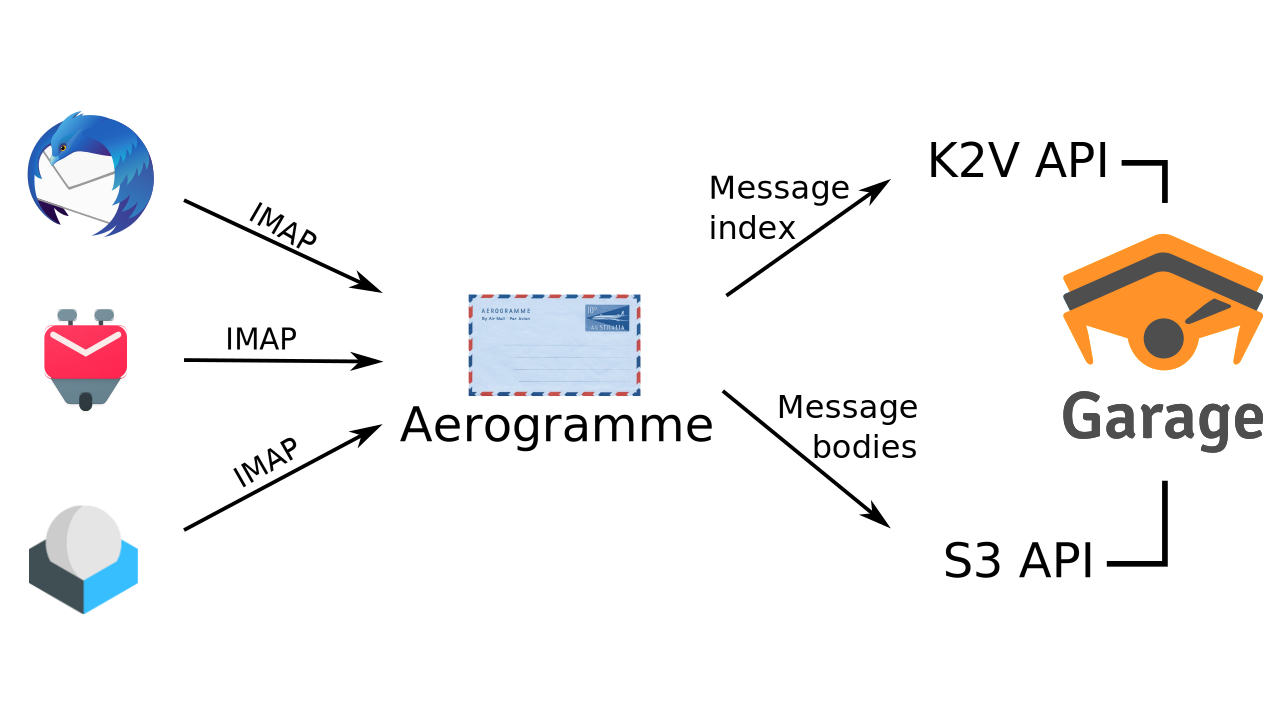
\includegraphics[width=.9\linewidth]{assets/aerogramme.png}}%
	\end{center}
\end{frame}

\begin{frame}
	\frametitle{Aerogramme data model}
	\begin{center}
		\only<1>{\includegraphics[width=.4\linewidth]{assets/aerogramme_datatype.drawio.pdf}}%
		\only<2->{\includegraphics[width=.9\linewidth]{assets/aerogramme_keys.drawio.pdf}\vspace{1em}}%
	\end{center}
	\visible<3->{Aerogramme encrypts all stored values for privacy\\
	(Garage server administrators can't read your mail)}
\end{frame}

\begin{frame}
	\frametitle{Different deployment scenarios}
	\begin{center}
		\only<1>{\includegraphics[width=.9\linewidth]{assets/aerogramme_components1.drawio.pdf}}%
		\only<2>{\includegraphics[width=.9\linewidth]{assets/aerogramme_components2.drawio.pdf}}%
	\end{center}
\end{frame}

\begin{frame}
	\frametitle{A new model for building resilient software}
	\begin{itemize}
		\item Design a data model suited to K2V\\
			{\footnotesize (see Cassandra docs on porting SQL data models to Cassandra)}
			\vspace{1em}
			\begin{itemize}
				\item Use CRDTs or other eventually consistent data types (see e.g. Bayou)
					\vspace{1em}
				\item Store opaque binary blobs to provide End-to-End Encryption\\
			\end{itemize}
			\vspace{1em}
		\item Store big blobs (files) in S3
			\vspace{1em}
		\item Let Garage manage sharding, replication, failover, etc.
	\end{itemize}
\end{frame}

\begin{frame}
	\frametitle{Research perspectives}
	\begin{itemize}
		\item Write about Garage's global architecture \emph{(paper in progress)}
			\vspace{1em}
		\item Measure and improve Garage's performances
			\vspace{1em}
		\item Discuss the optimal layout algorithm, provide proofs
			\vspace{1em}
		\item Write about our proposed architecture for (E2EE) apps over K2V+S3
	\end{itemize}
\end{frame}

\begin{frame}
	\frametitle{Where to find us}
	\begin{center}
			\includegraphics[width=.25\linewidth]{../../logo/garage_hires.png}\\
			\vspace{-1em}
		\url{https://garagehq.deuxfleurs.fr/}\\
		\url{mailto:garagehq@deuxfleurs.fr}\\
		\texttt{\#garage:deuxfleurs.fr} on Matrix

		\vspace{1.5em}
			\includegraphics[width=.06\linewidth]{assets/rust_logo.png}
			\includegraphics[width=.13\linewidth]{assets/AGPLv3_Logo.png}
	\end{center}
\end{frame}

\end{document}

%% vim: set ts=4 sw=4 tw=0 noet spelllang=en :
